\documentclass{article}
\usepackage[T1]{fontenc}
\usepackage{lmodern}
\usepackage{graphicx}
\usepackage{amsmath,amssymb}
\usepackage[a4paper,margin=2cm]{geometry}
\usepackage[absolute,overlay]{textpos}
\setlength{\TPHorizModule}{1mm}
\setlength{\TPVertModule}{1mm}
\usepackage[indonesian]{babel}
\usepackage{hyperref}
\setlength{\emergencystretch}{2em}
% unit: Halaman 38

\begin{document}

% === Halaman 38 (llm) ===

section{6. Kunci}

\begin{itemize}
    \item Agar enkripsi dan dekripsi hanya dapat dilakukan oleh dua pihak yang berkomunikasi, maka diperlukan \textbf{kunci} rahasia.
    \item Kunci adalah parameter yang digunakan di dalam enkripsi dan dekripsi\\
    Simbol: K ( K dapat berupa integer, string, alphanumeric, dsb )
\end{itemize}

\vspace{83.16mm}

\[ \text{Enkripsi: } E_K(P) = C \quad ; \quad \text{Dekripsi: } D_K(C) = P \]

\vspace{30mm}

\textbf{Prinsip Kherkoff}: semua algoritma kriptografi harus publik (tidak rahasia), hanya kunci yang harus rahasia.

% deskripsi: Diagram alir proses enkripsi dan dekripsi yang menunjukkan aliran dari Plainteks melalui proses Enkripsi (menggunakan Kunci) menjadi Cipherteks, lalu melalui proses Dekripsi (menggunakan Kunci) kembali menjadi Plainteks.
% bbox normalisasi: [0.1440, 0.4600, 0.8200, 0.7400]
\begin{textblock*}{141.96mm}(30.24mm,136.62mm)
\noindent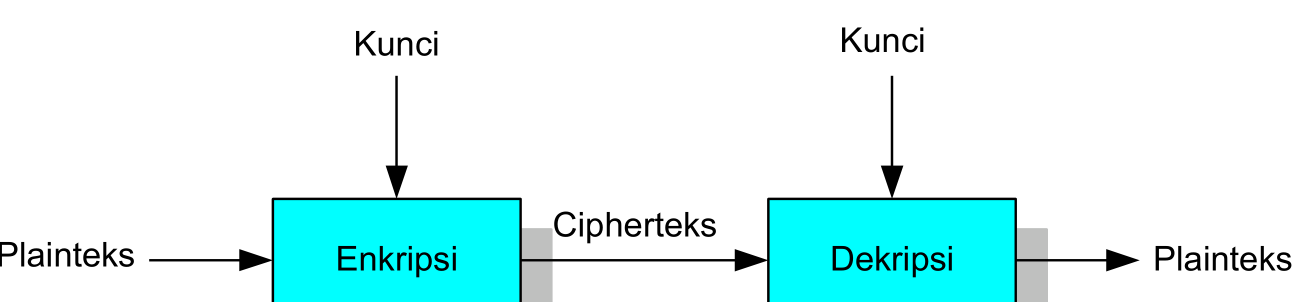
\includegraphics[width=141.96mm,height=83.16mm]{../../images/llm/page_038_img_01.png}%
\end{textblock*}

\end{document}
